\documentclass[11pt,a4paper]{article}

\usepackage[margin=2.2cm]{geometry}
\usepackage[T1]{fontenc}
\usepackage[utf8]{inputenc}
\usepackage[english]{babel}
\usepackage{lmodern}
\usepackage{microtype}
\usepackage{hyperref}
\usepackage{graphicx}
\usepackage{booktabs}
\usepackage{array}
\usepackage{longtable}
\usepackage{enumitem}
\usepackage{xcolor}
\usepackage{titlesec}
\usepackage{setspace}
\usepackage{float}

\hypersetup{
  colorlinks=true,
  linkcolor=blue,
  urlcolor=blue,
  citecolor=blue,
  pdftitle={SMTUC and Metrobus: A Visualization Study for Coimbra},
  pdfauthor={Project Group}
}

\setlength{\parindent}{0pt}
\setlength{\parskip}{0.65em}
\onehalfspacing
\titleformat{\section}{\large\bfseries}{\thesection}{0.6em}{}
\titleformat{\subsection}{\normalsize\bfseries}{\thesubsection}{0.6em}{}

\title{SMTUC and Metrobus: A Visualization Study for Coordinated Transit Planning in Coimbra}
\author{Author 1 \and Author 2}
\date{\today}

\begin{document}
\maketitle

\begin{abstract}
This report describes the final version of an interactive visualization project focused on public transport in Coimbra after the introduction of Metrobus. The goal is to help evaluate where SMTUC service overlaps with Metrobus, where service remains weak relative to population, and how the network behaves at specific times and stops. The project combines GTFS-based data preparation, geospatial analysis, and interactive visualizations implemented in Python with Plotly-based dashboards. The resulting application supports multiple analytical views, including population coverage, underservice scoring, overlap analysis, and timetable integration views for the Linha 54 corridor.
\end{abstract}

\section{Authors}
This project was developed by a two-person team. The report and the code should list the final authors here, together with institutional emails. At the time of writing, the report template keeps these fields as placeholders so the final submission can be completed with the correct names and contact details.

\section{Introduction}
Coimbra's transit system is currently shaped by the coexistence of SMTUC bus services and the Metrobus corridor. This creates a planning problem that is not only spatial but also temporal: some areas are already well served by overlapping modes, while other areas remain relatively underserved and may require intervention. The project addresses this problem by building a visual analytical environment that helps compare service redundancy, population exposure, and timetable coordination.

The main question is how SMTUC should adapt to Metrobus so that service is aligned with current demand and future mobility needs. The intended users are transit planners, instructors, and technically literate decision makers who need to inspect service gaps, identify overlapping corridors, and understand the timing relationship between modes. The project is not designed as a generic public-facing map only; it is also an analytical application that supports decision making through multiple linked views and derived metrics.

\section{Related Work}
The project was informed by examples of modern data journalism, transit mapping, and analytical dashboards that combine geographic context with service metrics. Inspiration came from interactive web visualizations that use choropleths, heatmaps, and layered maps to reveal structure in mobility systems. The design also follows standard visualization principles discussed in class, especially clarity of encoding, semantic color use, and the importance of combining overview and detail.

The implementation follows a Plotly-centered workflow so that the outputs remain easy to inspect in a browser and suitable for iterative exploration. Compared with static charts, the chosen approach allows hover interaction, dynamic filtering, linked summaries, and reusable HTML views.

\section{Design Requirements}
The visualization was designed around a small set of analytical goals. First, it should show where Metrobus and SMTUC overlap spatially and where they diverge. Second, it should show where population is high but service remains weak. Third, it should support timetable inspection for a representative corridor so that the interaction between bus and metro can be studied at specific times of day. Fourth, it should remain readable and lightweight enough to support repeated exploration.

These goals translated into requirements for geospatial views, time-based heatmaps, summary tables, and explanatory dashboards. The application had to support hover inspection, filtering through dashboard navigation, and clear labels in Portuguese for the final user-facing outputs. Good design practices also mattered: the views needed titles, legends, and a consistent color language so that higher deficiency or worse service could be read immediately.

\section{Data}
The project uses GTFS feeds for SMTUC, Metrobus, and supporting service data, together with a census-based geospatial dataset for population in BGRI units. The SMTUC data were cross-checked against the public static GTFS resource published on Dados.gov.pt for the Servicos Municipalizados de Transportes Urbanos de Coimbra, which provides an official public access point for the network feed. The population layer is read from a GeoPackage, while the transport layers are processed from GTFS text files such as stops, trips, routes, stop times, calendar, and calendar dates. The data model therefore combines tabular timetable data with geographic boundaries and point locations.

The repository contains a structured data folder with separate GTFS feeds and census data, while the outputs folder stores generated HTML dashboards and CSV summaries. During preparation, the data were normalized into reusable Python functions, and the geospatial layers were projected into a metric CRS for distance calculations. Population was merged with a derived underservice score that combines resident population and service departures. A separate procedure computes zones within a chosen radius around the stadium for the case study view.

\section{Exploratory Data Analysis}
EDA was used to understand both service structure and the shape of the derived indicators. For the transit side, the analysis focused on route overlap, stop density, timetable regularity, and temporal coincidence between bus and metro services. For the population side, the analysis investigated how population clusters relate to service availability and how underserved zones change when the catchment radius is expanded.

The output of EDA guided several decisions. Choropleth maps were selected because the main question is spatial and the underlying data are territorial. Heatmaps were used for timetable summaries because they reveal temporal patterns without forcing a one-dimensional ordering. The project also used derived indicators rather than raw counts only, because service analysis must account for both frequency and exposure. The most important derived metric is the underservice score, which expresses resident population relative to service departures and highlights areas where service is weaker relative to demand.

A second EDA result was that high-density service zones can become visually unreadable when all polygons and outlines are emphasized equally. This led to percentile-based color scaling, more restrained borders, and a stronger separation between the overview map and the stadium-focused case study. Another EDA outcome was that the analysis is more useful when the labels are translated into meaningful language rather than raw variable names. This is why the final dashboards use Portuguese labels such as "Índice de Subserviço" and "Espera Média (min)".

\begin{figure}[H]
\centering
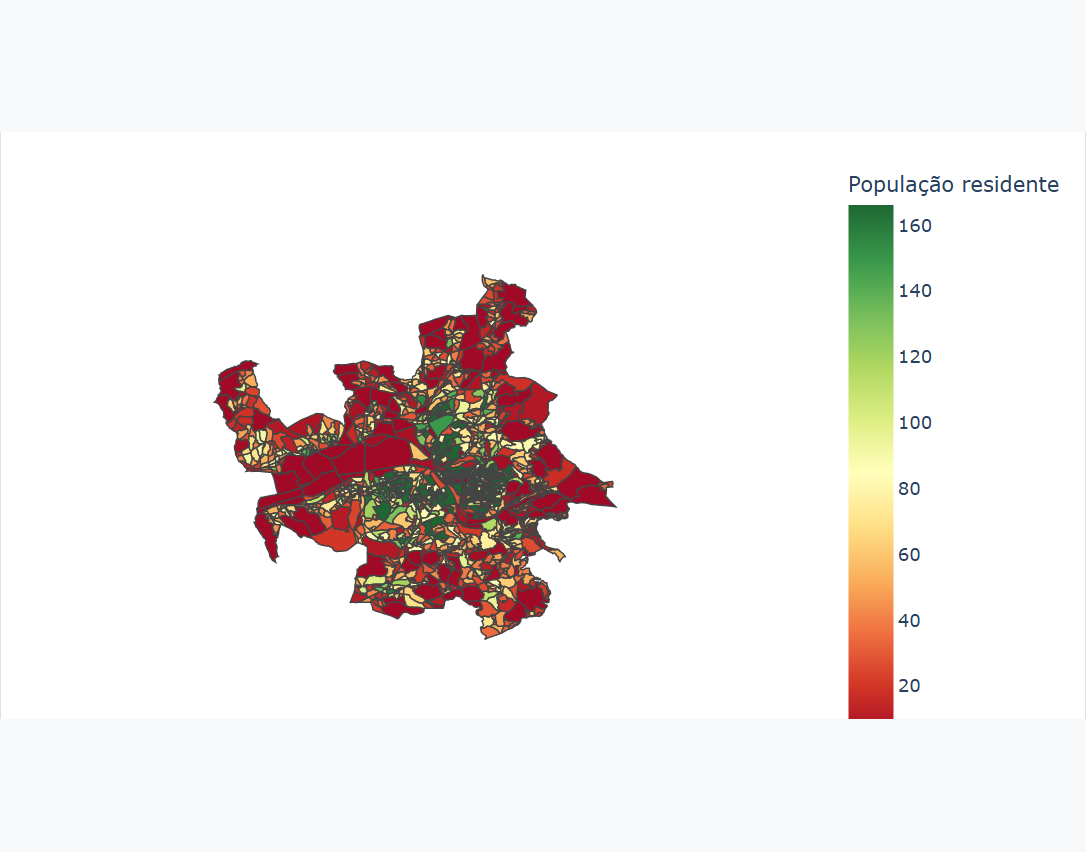
\includegraphics[width=0.95\linewidth,height=5.2cm,keepaspectratio]{figures/population_heatmap.png}
\caption{Population heatmap used to inspect concentration patterns across BGRI units.}
\label{fig:overview-suggested}
\end{figure}

\begin{figure}[H]
\centering
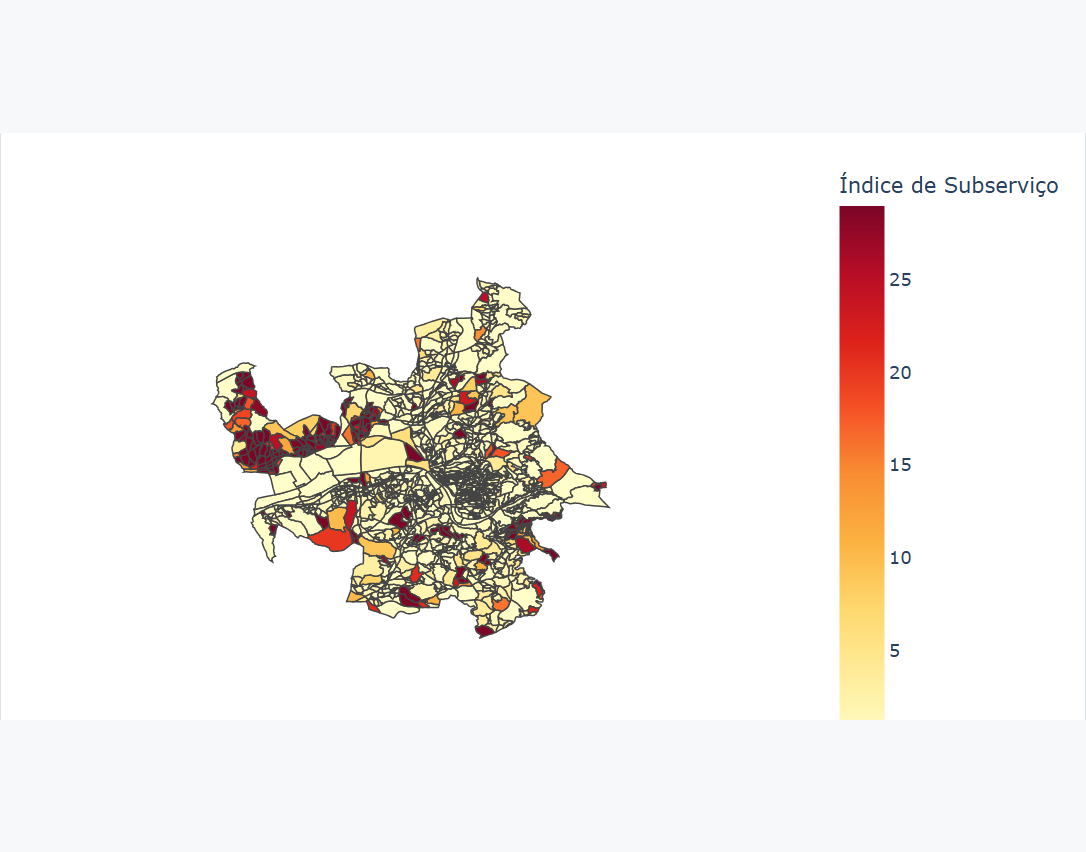
\includegraphics[width=0.95\linewidth,height=5.2cm,keepaspectratio]{figures/population_underservice.png}
\caption{Underservice choropleth showing the derived service pressure score.}
\label{fig:underservice-suggested}
\end{figure}

\begin{figure}[H]
\centering
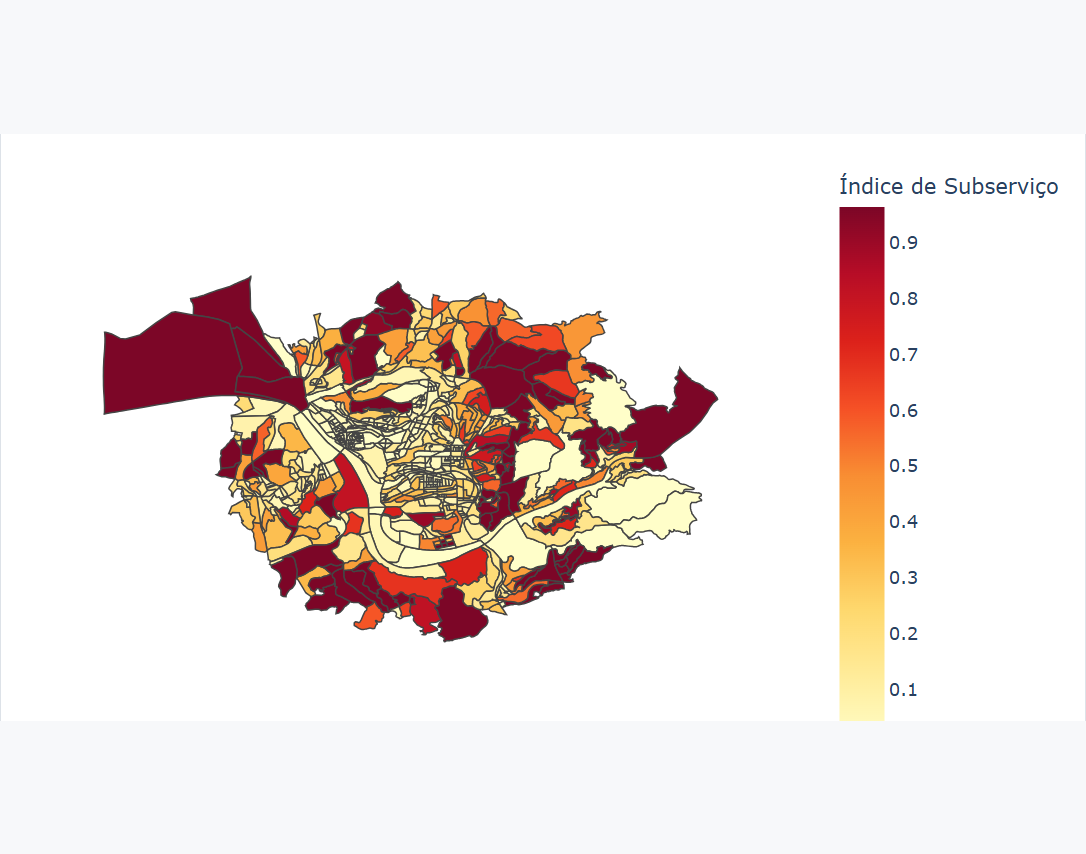
\includegraphics[width=0.95\linewidth,height=5.2cm,keepaspectratio]{figures/population_stadium.png}
\caption{Stadium case study focused on the 2 km catchment around the stadium.}
\label{fig:stadium-suggested}
\end{figure}

\section{Design}
The visual design follows a layered structure. The main dashboard provides a high-level entry point, while the population dashboard and the integration dashboards expose the detailed analyses. The color choice is semantic: better or lighter conditions are shown with cooler or lighter tones, while worse conditions use warmer and more urgent tones. For the underserved maps, a sequential palette that transitions from green to red was chosen so that higher scores immediately read as more problematic. For the integration heatmaps, warm colors were also used to emphasize higher values.

The interaction design is intentionally simple but effective. Hover details reveal the data behind each map. Tabs and embedded panels allow users to switch between views without losing context. In the integration views, linked summary statistics and heatmaps make it possible to connect waiting times, coverage, and temporal performance within one corridor. The report and dashboards prioritize legibility, with clear titles, compact legends, and readable labels in the final language of the submission.

\section{Implementation}
The application is implemented in Python and organized into modules for GTFS processing, overlap analysis, population analysis, and visualization generation. The visual layer uses Plotly for the interactive charts and HTML generation, while geospatial operations rely on GeoPandas and related spatial tooling. The generated dashboards are stored under the outputs directory so that they can be opened directly in a browser.

The implementation separates the analytical functions from the presentation functions. Population maps are generated from a common choropleth helper, while the integration views build timetable heatmaps, waiting-time bar charts, and a final temporal equity heatmap. The system also includes reusable scripts for regenerating the population and integration dashboards. Tests cover the main outputs and verify that the HTML artifacts are generated correctly.

The current codebase is structured to support continued refinement. This matters because the project is not just a one-off rendering exercise. It is a reproducible visualization workflow where data preparation, derived metrics, and rendered outputs can be regenerated as the underlying feeds or assumptions change.

\begin{figure}[H]
\centering
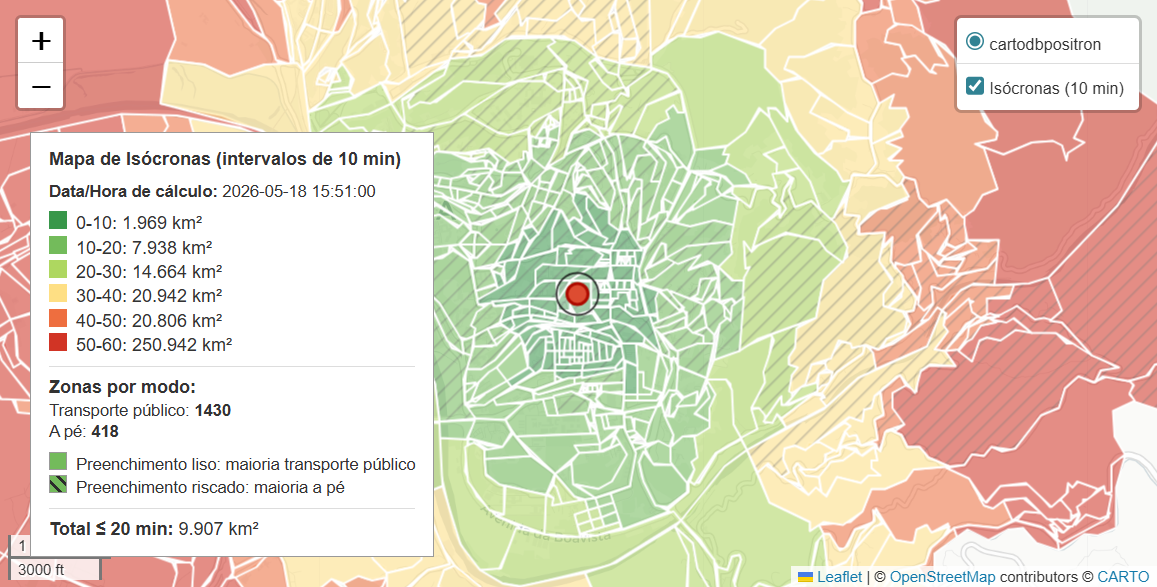
\includegraphics[width=0.95\linewidth,height=6cm,keepaspectratio]{figures/overlap_reachability.png}
\caption{Interactive reachability map used to inspect transit overlap and spatial accessibility.}
\label{fig:architecture-suggested}
\end{figure}

\section{Evaluation}
The visualization was evaluated through iterative inspection of the generated dashboards and through test-driven regeneration of the outputs. The main practical criterion was whether the figures stayed readable and whether the encoded metrics matched the analytical questions. This led to several revisions in the report and code, including label translation, color adjustments, and tighter dashboard organization.

The final prototype performs well at revealing where the network overlaps, where service is weak relative to population, and how the Linha 54 corridor behaves over time. It is particularly effective when used as a guided analytical tool rather than as a passive map. Its main limitations are that it still depends on curated datasets and that some GTFS feeds may be incomplete or inconsistent. The current version also remains a browser-based prototype rather than a fully polished production system.

\section{Critical Reflection}
The project demonstrates that a transit visualization can be useful only if it combines spatial, temporal, and demographic dimensions in a coherent way. A single map is not enough to explain the system. The derived indicators, linked dashboards, and corridor-level summaries make it possible to inspect redundancy, weak service, and timing relationships in one workflow.

The final result is effective for identifying service gaps and for comparing SMTUC against Metrobus, but it could still improve in three areas. First, the data pipeline could be made more robust, especially for missing GTFS fields and stop geometry inconsistencies. Second, the application could expose more direct interaction, such as range filters or brushing across views. Third, the report could be expanded with user feedback or a structured evaluation study to better assess decision usefulness.

Despite these limits, the project already supports the core analytical questions that motivated it. It shows where the network is redundant, where population pressure is high, and how a representative corridor behaves across the day. This makes the visualization useful both as a communication tool and as a decision-support prototype.

\section{Conclusion}
This project produced an interactive visualization environment for SMTUC and Metrobus in Coimbra, with emphasis on overlap, underserved areas, and timetable coordination. The final implementation is reproducible, modular, and grounded in real transit and population data. It shows how Plotly-based dashboards can be used for analytical transportation visualization without sacrificing clarity or flexibility.

Future work should improve data completeness, introduce richer linking between views, and incorporate feedback from intended users. A more mature version could also provide a more explicit Dash application wrapper, additional filtering controls, and a stronger evaluation component.

\begin{thebibliography}{9}

\bibitem{gtfs}
Google.
\newblock General Transit Feed Specification Reference.
\newblock \url{https://gtfs.org/}, accessed in 2026.

\bibitem{dadosgovsmtuc}
Dados.gov.pt.
\newblock GTFS Estaticos Servicos Municipalizados de Transportes Urbanos de Coimbra.
\newblock \url{https://dados.gov.pt/pt/datasets/gtfs-estaticos-servicos-municipalizados-de-transportes-urbanos-de-coimbra/#/resources/e9b422cc-75bd-4ccf-8a01-50e121d6e423}, accessed in 2026.

\bibitem{plotly}
Plotly Technologies Inc.
\newblock Plotly Python Graphing Library.
\newblock \url{https://plotly.com/python/}, accessed in 2026.

\bibitem{geopandas}
GeoPandas Developers.
\newblock GeoPandas Documentation.
\newblock \url{https://geopandas.org/}, accessed in 2026.

\bibitem{census}
Statistics Portugal.
\newblock Census and BGRI reference data.
\newblock \url{https://www.ine.pt/}, accessed in 2026.

\end{thebibliography}

\clearpage
\begin{figure}[H]
\centering
\begin{minipage}[t]{0.48\textwidth}
\centering
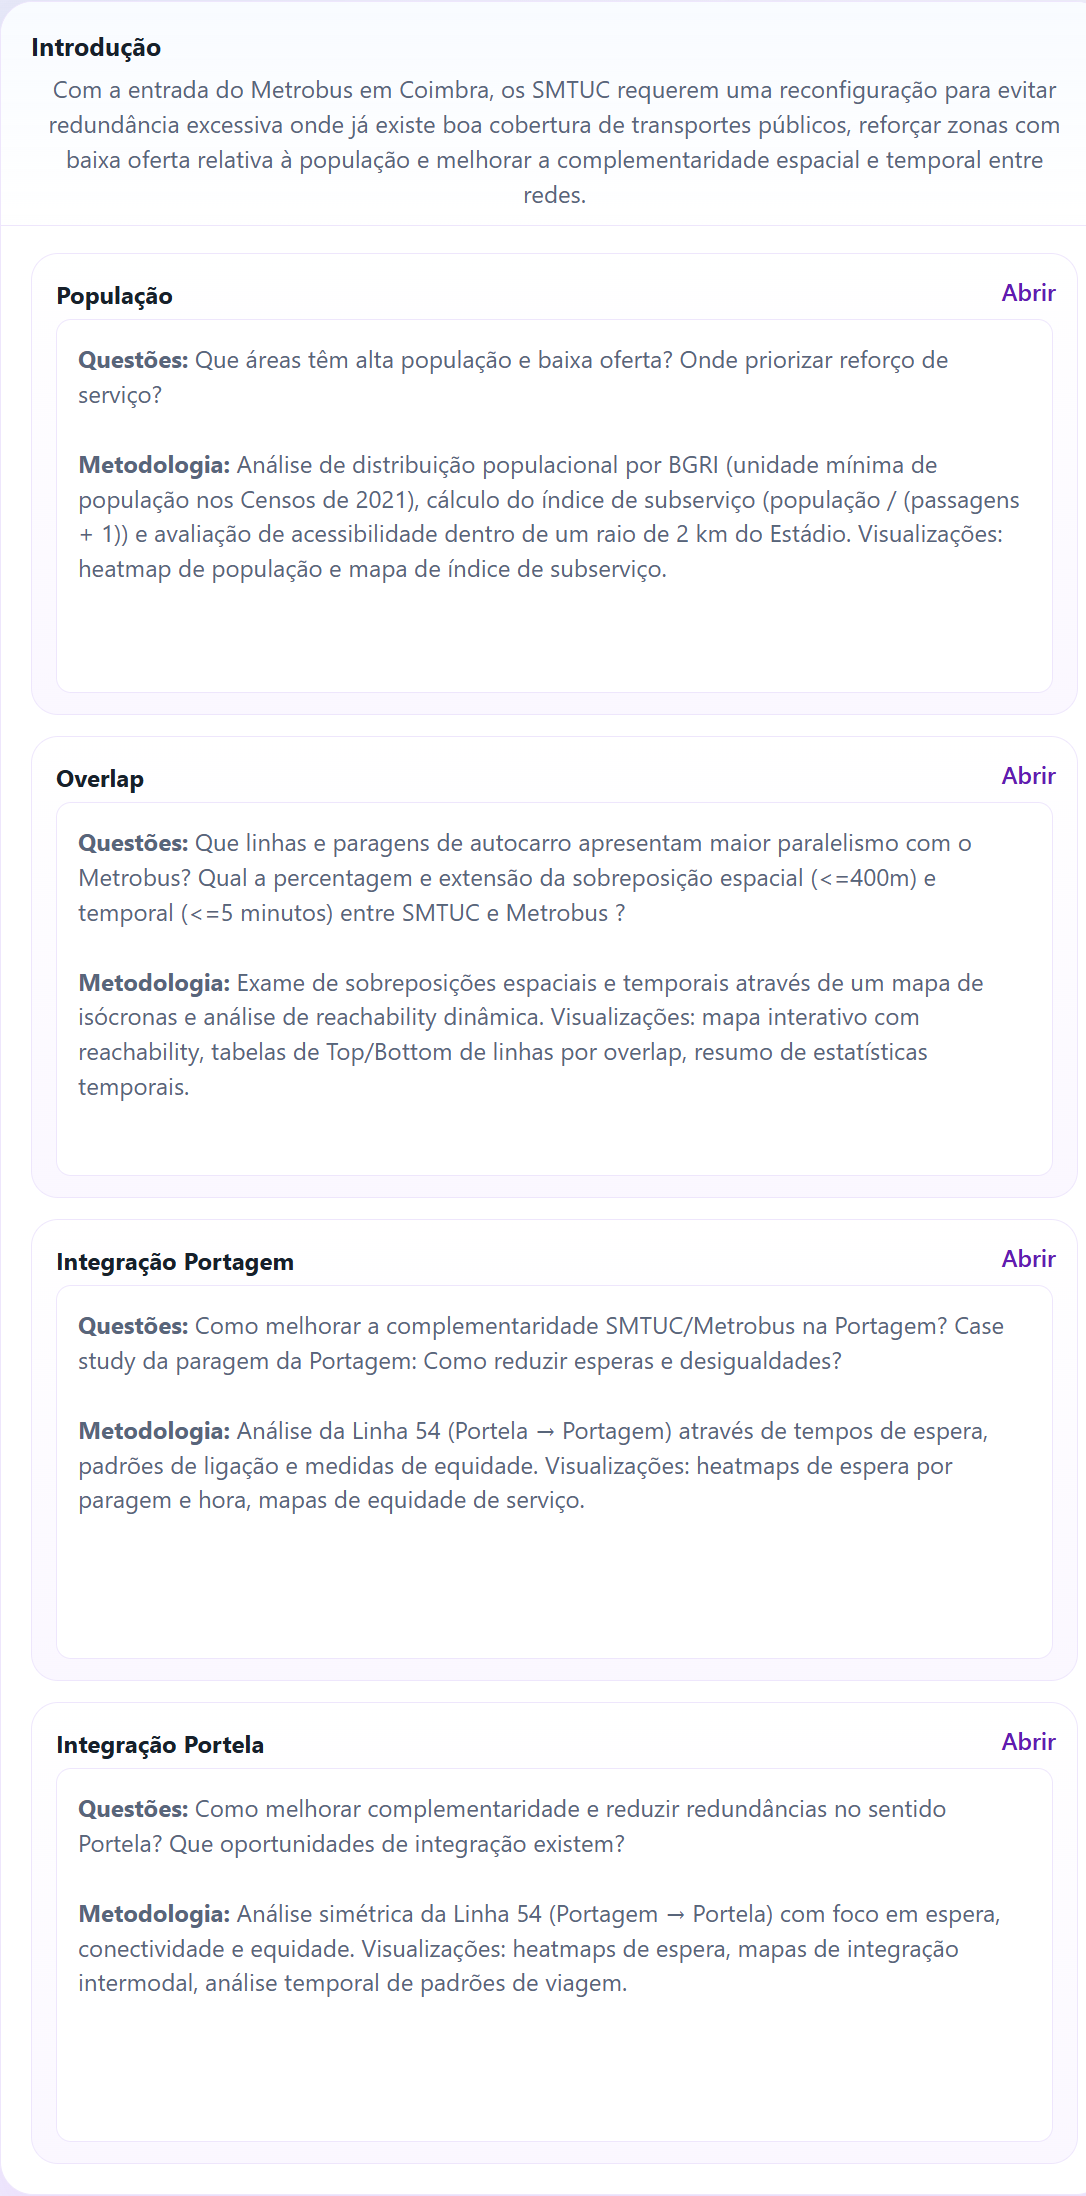
\includegraphics[width=\linewidth,height=0.72\textheight,keepaspectratio]{figures/summary_page.png}
\caption{Summary page used as the entry point to the analytical application.}
\label{fig:summary-page-final}
\end{minipage}\hfill
\begin{minipage}[t]{0.48\textwidth}
\centering
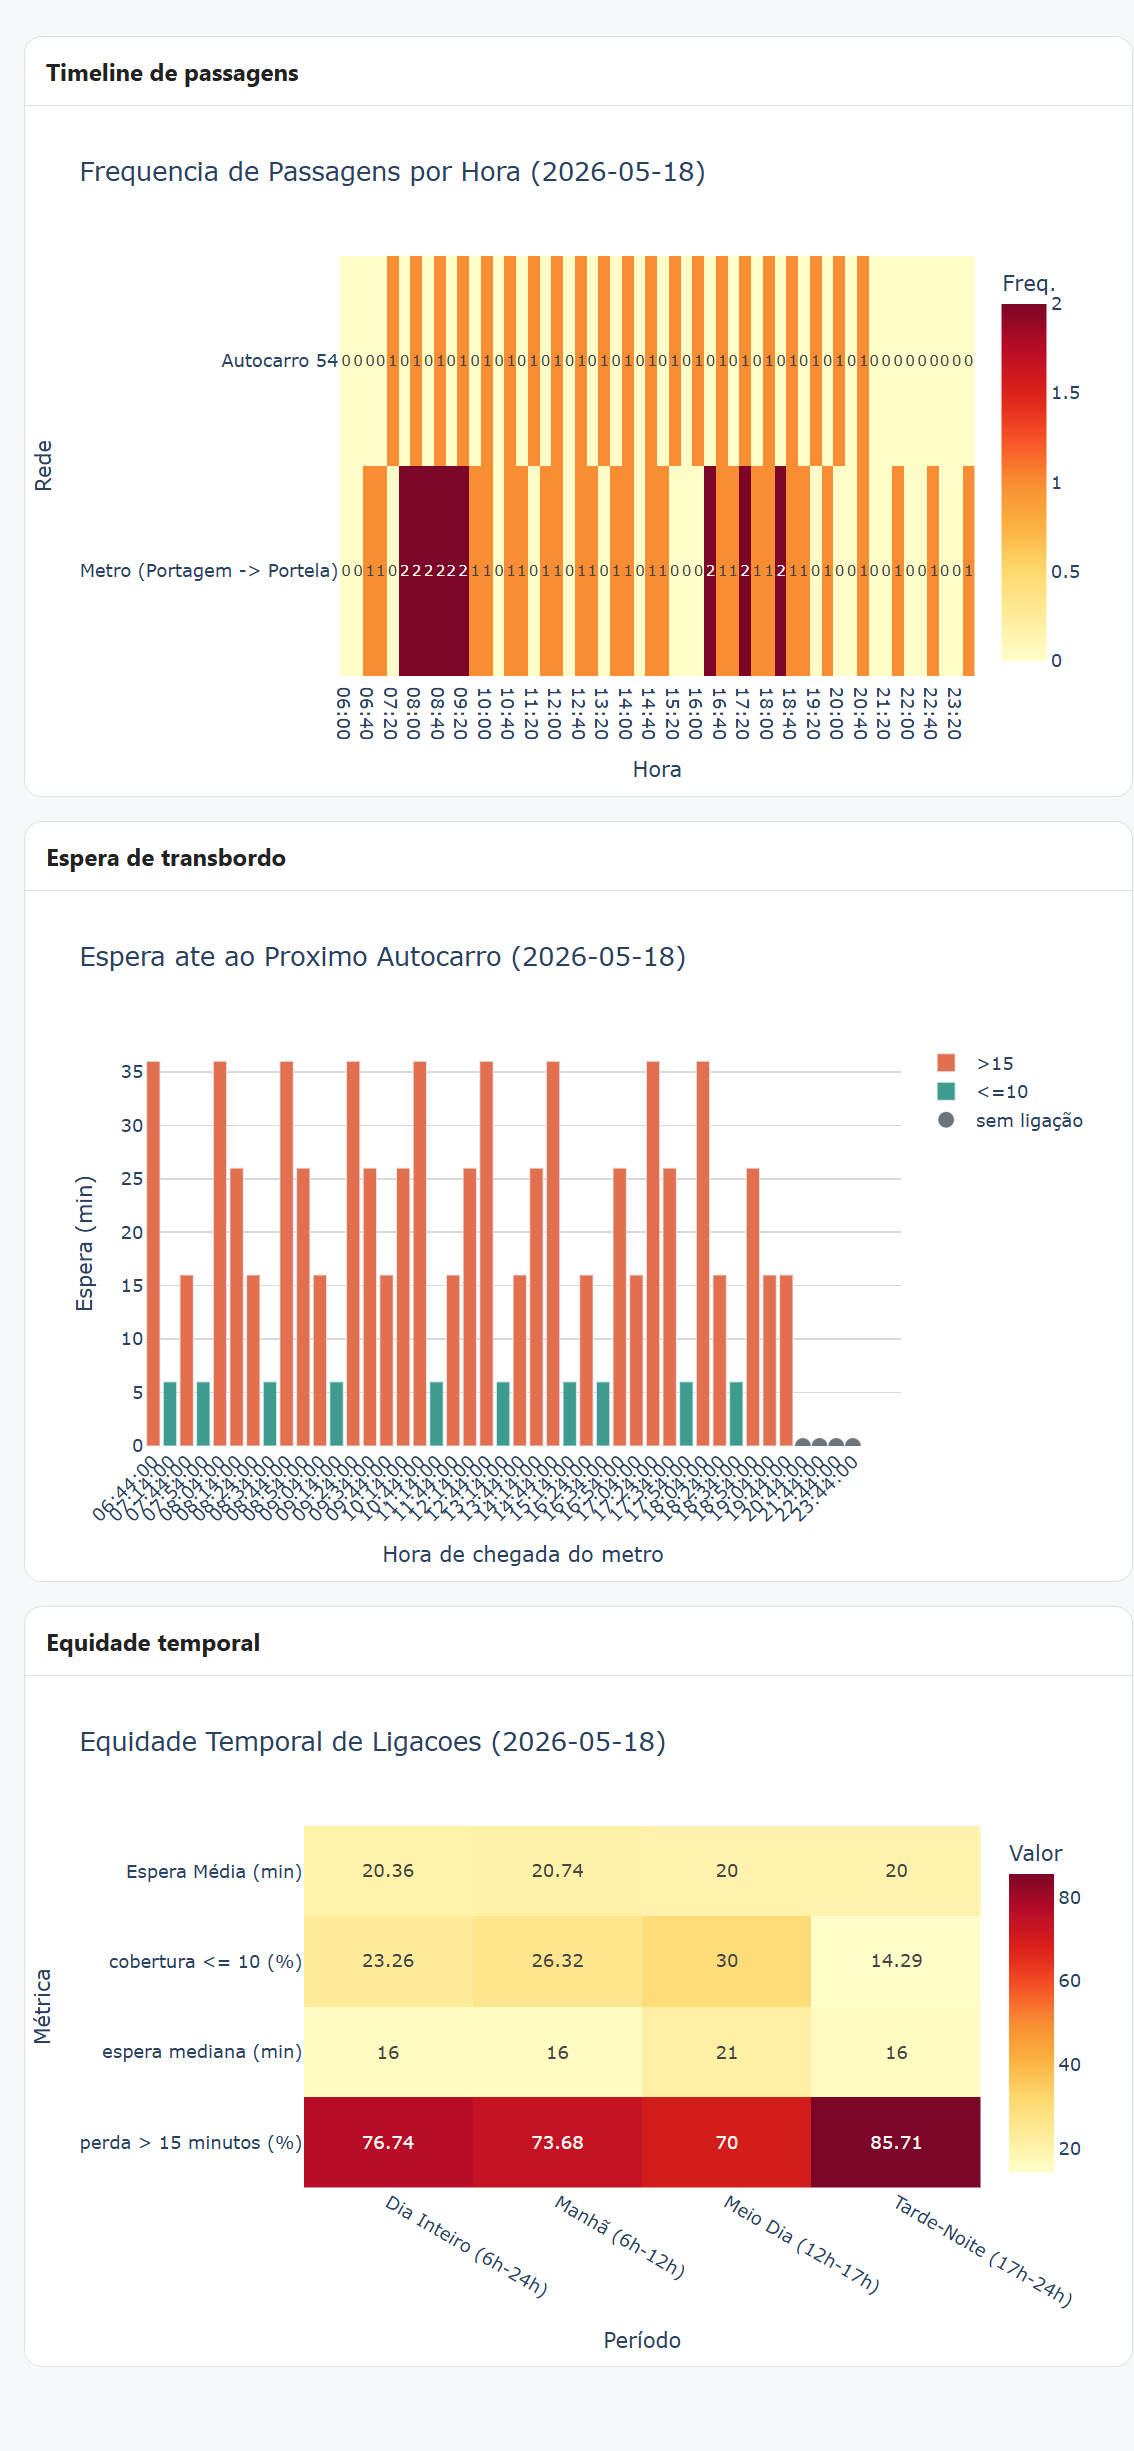
\includegraphics[width=\linewidth,height=0.72\textheight,keepaspectratio]{figures/integration_portela.png}
\caption{Integration dashboard for Linha 54 showing timetables, waiting times, and temporal equity.}
\label{fig:integration-portela-final}
\end{minipage}
\end{figure}

\end{document}
